% !TEX root = ../SU2-Scitech15.tex

\section{Results}
First executive summary of the results a table and couple figures that show everyone we varied and did. For instance a figure could look like this \cref{fig:Cd_convergence}
Second, organize results subsections either by grid or angle of attack, whichever makes more sense once we have the results.
Third, show validation results for a representative case.
Figures and tables in this section should address questions such as: how do variation in the forces due to changing grids compare with changing the parameters? Which parameters change speed of convergence? Which parameters change value to which we converge? ...

\begin{figure}
  \centering
  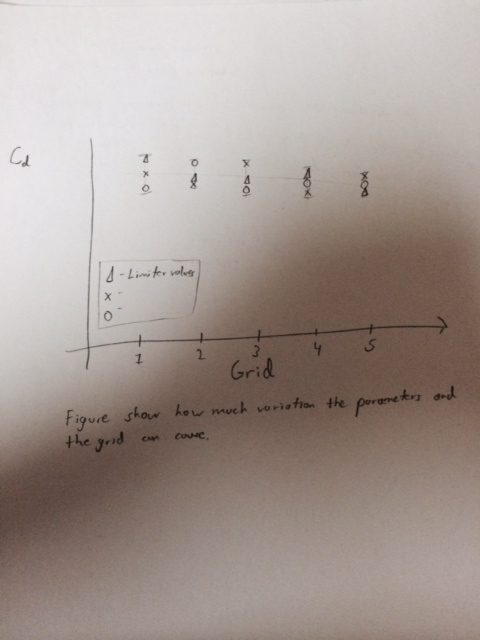
\includegraphics[width=0.5\textwidth]{./fig/cd_convergence}
  \caption{Drag coefficient convergence and variation.}
  \label{fig:Cd_convergence}
\end{figure}

Also, a sample table \cref{tab:sample_table} to be used as a template.
\begin{table}
  \centering
  \begin{tabular}{ccccccc} \\ \toprule
  Grid & npoints x 1000 & points airfoil & y+ & \#points in BL & growth rate  \\ \midrule
  1 (1793 x 513) & 920 & 1025 & 0.09 & 212 & 1.035\\
  2 (897 x 257) & 231 & 513 & 0.18 & 107 & 1.071\\
  3 (449 x 129) & 58 & 257 & 0.36 & 54 & 1.148\\
  4 (225 x 65) & 14.6 & 129 & 0.72 & 27 & 1.319\\
  5 (113 x 33) & 3.73 & 65 & 1.44 & 14 & 1.749\\ \bottomrule
  \end{tabular}
  \caption{Rough description of the grids. Double check when we get the grids from Francisco.  I(Santiago) calculated y+ and \#points in BL assuming a flat plate at the given Reynolds. The growth rate was backed out of the description of the grids in NASA. The grids might be extruded differently. In any case this is a table that can be used as a sample.}
  \label{tab:sample_table}
\end{table}
